\documentclass[12pt]{article}
\usepackage{color}
\usepackage[margin=3cm]{geometry}
\usepackage{graphicx}
\graphicspath{{C:/Users/admin/Downloads/}}
\DeclareGraphicsExtensions{.jpg}
%\usepackage[utf8]{inputenc}
%\usepackage[backend=biber,style=alphabetic,sorting=ynt]
%{biblatex}
%\addbibresource{201601004.bib}
\usepackage{draftwatermark}
\SetWatermarkText{POOJAN DHAMELIYA}
\SetWatermarkScale{0.5}
\usepackage{hyperref}
\usepackage{times}
\begin{document}
\title{\textcolor{red}{CHEMICAL KINETICS MODEL}}
\begin{center}
\Huge
 {\bf \textcolor{red}{ 
{ DIWALI  ASSIGNMENT OF CALCULUS }       \\
 }
}
\vspace{2 cm}
\Large\bf
{ Assigned by : Professor Manish K Gupta}  \\
\huge\bf { COURSE      : SC 107   \\
  Calculus. Where are you?\\
  FALL 2016    \\
  DA-IICT      \\
  GANDHINAGAR  \\
}
\vspace{5 cm}
\LARGE {\it
{ 
  Made by: POOJAN DHAMELIYA   \\
  ID  : 201601450 \\
}
}
\end{center}
\author{
         POOJAN DHAMELIYA\\
         201601450,\\
         DAIICT,\\
         GANDHINAGAR,\\
         INDIA\\
         \texttt{201601450@daiict.ac.in}
      }  
\date{\today}
\maketitle
\begin{abstract}
\textcolor{red}
{
\large
{
In this article, I shall discuss  the way of solving the classical
 `CHEMICAL KINETICS PROBLEM'.It is used to determine the rate law of chemical reactions in which differential equation plays a major role to conclude it.
}
}
\end{abstract}

  \begin{center}
  
\includegraphics[scale=1.0]{201601450}
\end{center}
\newpage
\section{\textcolor{red}{INTRODUCTION}}
\textsf
Chemical kinetics, also known as reaction kinetics, is the study of rates of chemical processes. Chemical kinetics includes investigations of how different experimental conditions can influence the speed of a chemical reaction and yield information about the reaction's mechanism and transition states, as well as the construction of mathematical models that can describe the characteristics of a chemical reaction.

        Determining rates of chemical reactions is a crucial first step in the design of any commercial chemical process, so this is an area of particular interest to chemists and chemical engineers.   
                                           


\section{\textcolor{red}{ THE FIRST ORDER CHEMICAL RATE EQUATION }}
\textsf
From Experimental results,it was found that chemical rate equation is in the form of differential equation.
\subsection{\textcolor{blue}{DEPENDS ON ONE PRODUCT}}
\textsf
		For example, A stirred vessel contains a solution of a chemical substance W, which decays spontaneously to form products. If we let w(t) represent the concentration of species W in the vessel as a function of time, then it has been found experimentally that the rate at which W decays is proportional to its concentration. In mathematical terms, this means that w(t) satisfies a differential equation of the form 
\textcolor{blue}{$\frac{d}{dt}\,w(t)=-k\,w(t)$}.\\
\subsection{\textcolor{blue}{DEPENDS ON MORE THAN ONE PRODUCTS}}
\textsf
As a more interesting example, suppose that two substances, Y and Z, combine in a chemical reaction to form a substance X. We will assume that the rate at which the molecules of X are formed is proportional to the product of the concentrations of Y and Z at time t. Let \textcolor{blue}{$x(t),y(t),$}and \textcolor{blue}{z(t)} be,,respectively, the concentrations of chemicals X, Y, and Z present at time t. Then we have the rate law 

$\textcolor{blue}{\frac{d}{dt}\,x(t)=k\,y(t)\,z(t).}$

\newpage
\section{\textcolor{red}{ SOLUTION OF FIRST ORDER RATE EQUATION }}
\textsf
This type of differential equation can be solved by separable variables methods.
\subsection{\textcolor{blue}{ DEPENDS ON ONE PRODUCT }}
\large
{
\textcolor{blue}{$$ \frac{d\,w(t)}{w(t)}=-k\,dt$$
$$\int{\frac{d\,w(t)}{w(t)}}=\int{-k\,dt}$$
$$log{|w(t)|}=-kt+\kappa$$
$$w(t)=-e^{-kt}e^{\kappa}$$
$$w(t)=-\kappa\,e^{kt}$$}}
THE PROBLEM IS SOLVED.
\subsection{\textcolor{blue}{DEPENDS ON MORE THAN ONE PRODUCTS }}
\textsf
The next step is to express $y(t)$ and $z(t)$ in terms of $x(t)$ and then substitute the resulting expressions into the rate law to get a differential equation involving only $x(t)$. This is done as follows:

       We are assuming that one molecule of Y and one molecule of Z combine to form one molecule of X and that there is no X present initially. That is, for every molecule of X formed, one molecule of Y and one molecule of Z must be consumed. This means that $\textcolor{blue}{y(t)=y(0)-x(t)}$ and $\textcolor{blue}{z(t)=z(0)-x(t)}$, where $\textcolor{blue}{y(0)}$ and $\textcolor{blue}{z(0)}$ are the initial concentrations of Y and Z. Thus we have 
       
     \textcolor{blue}{${\mathrm{\frac{d}{dt}\,x(t)=k\,(y(0)-x(t))\,(z(0)-x(t))}}$}
     This is a separable differential equation that can be solved using the technique described above.

THE PROBLEM IS SOLVED.

\newpage
\section{\textcolor{red}{THE SECOND ORDER CHEMICAL RATE EQUATION}}
\textsf
  		The equation of second order rate equation is:
  	
  		(1)When the product is same
  		\textcolor{blue}{$$\frac{d\,[A]}{dt}=-k\,{[A]}^2$$}
  		
  		(2)When the product are different
  		\textcolor{blue}{$$\frac{d\,[A]}{dt}=-k\,[A]\,[B]$$}
\section{\textcolor{red}{THE SOLUTION OF SECOND ORDER RATE EQUATION}}
\subsection{\textcolor{blue}{FOR ONE PRODUCT}}
\textsf
 		Since we are interested in the change in concentration of A over a period of time, we integrate between t=0 and  t=t , the time of interest.
 		\textcolor{blue}{$$\int_{{[A]}_0}^{{[A]_t}}\frac{d[A]}{{[A]}^2}=-k\int_{0}^{t}dt$$}
 		To solve this, we use the following rule of integration (power rule):
 		\textcolor{blue}{$$\int{\frac{dx}{x^2}}=-\frac{1}{x}+\kappa$$}
 		We then obtain integrated rate equation.
 		\textcolor{blue}{$$\frac{1}{{[A]}_t}-\frac{1}{{[A]}_0}=kt$$}
 		Upon rearrangement of the integrated rate equation, we obtain an equation of the line:
 		\textcolor{blue}{$$\frac{1}{{[A]}_t}=kt+\frac{1}{{[A]}_0}$$}
\newpage
\subsection{\textcolor{blue}{FOR TWO PRODUCTS}}
\textsf         
           This situation that the initial concentration of the two reactants are not equal.Let x be the concentration of each species reacted at time t .
           Let \textcolor{blue}{${[A]}_0=a$} and \textcolor{blue}{${[B]}_0=b$},then \textcolor{blue}{$[A]=a-x;[B]=b-x$}.The expression of rate law becomes;
           \textcolor{blue}{$$-\frac{dx}{dt}=-k\,({[A]}_0-x)\,({[B]}_0-x)$$} 
           which can be rearranged as
           \textcolor{blue}{$$\frac{dx}{({[A]}_0-x)\,({[B]}_0-x)}=k\,dt$$}
           We integrate between t=0 and t,
           \textcolor{blue}{$$\int_{0}^{x}\frac{dx}{({[A]}_0-x)\,({[B]}_0-x)}=k\,\int_{0}^{t}\,dt$$}
           To solve this integration,we can use the method of partial fractions.
           \textcolor{blue}{$$\int_{0}^{x}\frac{1}{(a-x)\,(b-x)}\,dx=\frac{1}{b-a}\,(ln{\frac{1}{a-x}}-ln{\frac{1}{b-x}})$$}
           Evaluating the integral gives us:
           \textcolor{blue}{$$\int_{0}^{x}\frac{dx}{({[A]}_0-x)\,({[B]}_0-x)}=\frac{1}{{[B]}_0-{[A]}_0}\,ln{\frac{[B]\,{[A]}_0}{[A]\,{[B]}_0}}$$}
           We then obtain the integrated rate equation (under the condition that [A] and [B] are not equal).
           \textcolor{blue}{$$\frac{1}{{[B]}_0}-{[A]}_0\,ln{\frac{[B]\,{[A]}_0}{[A]\,{[B]}_0}}=k\,t$$}
           Upon rearrangement of the integrated rate equation, we obtain:
           \textcolor{blue}{$$ln{\frac{[B]\,{[A]}_0}{[A]\,{[B]}_0}}=k\,({[B]}_0-{[A]}_0)\,t$$}
           Hence, from the last equation, we can see that a linear plot of \textcolor{blue}{$ln{\frac{{[A]}_0\,[B]}{[A]\,{[B]}_0}}$} versus time is characteristic of second-order reactions.
           \newpage
           \begin{center}
  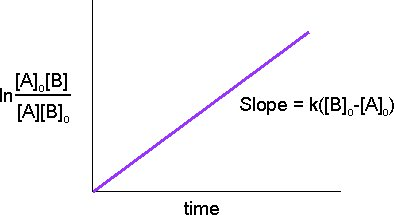
\includegraphics[scale=1.0]{poojan}
\end{center}
           This graph can be used in the same manner as the graph in the section above or written in the other way:
           \textcolor{blue}{$$ln{\frac{[A]}{[B]}}=k\,({[A]}_0-{[B]}_0)\,t+ln{\frac{{[A]}_0}{{[B]}_0}}$$}
         in form \textcolor{blue}{$y=a\,x+b$} with slope of \textcolor{blue}{$a=k\,({[B]}_0-{[A]}_0)$} and a y-intercept of \textcolor{blue}{$b=ln{\frac{{[A]}_0}{{[B]}_0}}$}.
         
         THE PROBLEM IS SOLVED.
         \newpage
\section{\textcolor{red}{ APPLICATION }}
\textsf
The mathematical models that describe chemical reaction kinetics provide chemists and chemical engineers with tools to better understand and describe chemical processes such as food decomposition, microorganism growth, stratospheric ozone decomposition, and the complex chemistry of biological systems. 

        These models can also be used in the design or modification of chemical reactors to optimize product yield, more efficiently separate products, and eliminate environmentally harmful by-products. When performing catalytic cracking of heavy hydrocarbons into gasoline and light gas, for example, kinetic models can be used to find the temperature and pressure at which the highest yield of heavy hydrocarbons into gasoline will occur.
        
       
\section{\textcolor{red}{CONCLUSION}}
\textbf
Due to this,we are able to find the rate at which we will get the products and also the quantity needed of reactants to satisfy our required amount of product.
 
        Thus, it will be helpful in predicting about the cost of reactants as we are able to guess about the quantity needed.
        \cite{1}
        \cite{2}
        \cite{3}
        \cite{4}
\newpage        
 
 
 
        
\bibliographystyle{plain}
\bibliography{201601450} 


\fontsize{50}{50}\selectfont{ THANK  YOU !!!}
\end{document}